%-------------------------------------------------------------------------
% Design Project Input/Output Module Description
%-------------------------------------------------------------------------

\section{Printer Output Module}
\label{sec-output-printer}

This printer output module enables your IoT device to print a paper copy of
collected/processed data for the end-user.  The printer is a thermal receipt
printer, similar to what is in most retail stores.  A thermal printer works by
selectively heating thermochromic paper (the receipt paper).  Heated sections of
paper turn black, creating the desired text or image, such as a barcode.

We'll be using the Arduino to control the printer.  However, because the
printer's thermal print head needs to be hot to work, it requires its own power
supply.  The printer comes with its own wall-wart power supply, which you should
plug into the barrel connector to screw-down terminal converter.  Ensure that
positive (red) is connected to the \texttt{+} and negative (black) is connected
to the \texttt{-} as shown below:

\begin{center}
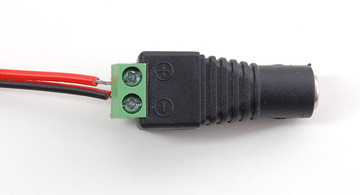
\includegraphics[width=2in]{components_poweradapt.jpg}
\end{center}

The printer has small plugs on the bottom: a 2-pin (power) and a 3-pin (data).
You'll hook up the power cable to the 2-pin plug (red/black) and hook that up to
the barrel connector converter (shown above).  The data cable connects 3-pin
connector on one end and to the Arduino for control, as shown below:

\begin{itemize}
\item Green: Digital Pin 5
\item Yellow: Digital Pin 6
\item Black: GND Pin
\end{itemize}

\begin{center}
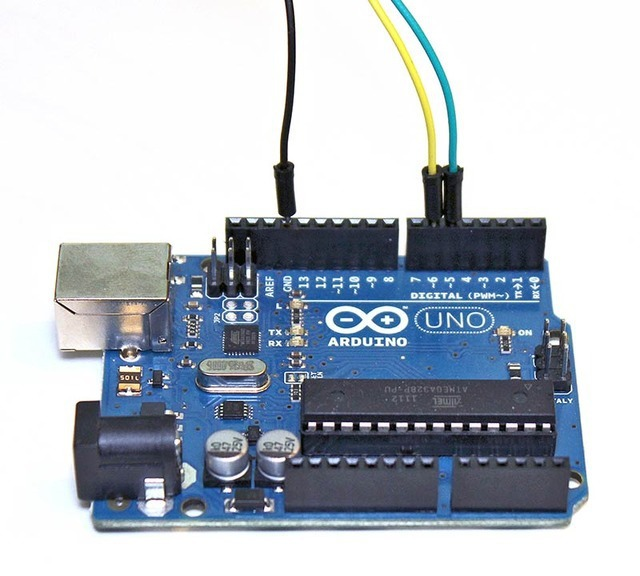
\includegraphics[width=4in]{components_printer-wiring.jpg}
\end{center}

\newpage

Using the printer is as simple as follows:

\begin{Verbatim}[gobble=3,fontsize=\small]
    #include "SoftwareSerial.h"
    #include "Adafruit_Thermal.h"
    #include <avr/pgmspace.h>

    int printer_RX_Pin = 5;  // This is the green wire
    int printer_TX_Pin = 6;  // This is the yellow wire

    Adafruit_Thermal printer(printer_RX_Pin, printer_TX_Pin);

    void setup(){
      Serial.begin(9600);
      pinMode(7, OUTPUT); digitalWrite(7, LOW); // To also work w/IoTP printer
      printer.begin();

      // The following function calls are in setup(), but do not need to be.
      // Use them anywhere!  They're just here so they're run only one time
      // and not printed over and over.
      // Some functions will feed a line when called to 'solidify' setting.
      // This is normal.

      //Hello World        
      print.println("Hello World!")

      // Set text justification (right, center, left) -- accepts 'L', 'C', 'R'
      printer.justify('R');
      printer.println("This Text Right Justified");
      printer.justify('C');
      printer.println("This Text Center Justified");
      printer.justify('L');
      printer.println("This Text Left Justified");

      // Set type size, accepts 'S', 'M', 'L'
      printer.setSize('L');
      printer.println("Large Text"); // Print line
      printer.setSize('M');
      printer.println("Medium Text");
      printer.setSize('S');
      printer.println("Small Text");

      printer.feed(1);

      printer.sleep();      // Tell printer to sleep
      printer.wake();       // MUST call wake() before printing again, even if reset
      printer.setDefault(); // Restore printer to defaults
    }

    void loop() {
    }
\end{Verbatim}
